The value reported here agrees with the two existing measurements of
the Yb/Sr ratio at the level set by the redefinition roadmap
(Figure~\ref{fig:compare}a). Relative to the NIST--JILA value
\refNistV(\refNistU)~\citep{aeppli2026nist}, our central value differs
by $\dVsNistE$; relative to the European-network value
\refEuV(\refEuU)~\citep{pizzocaro2026european}, it differs by
$\dVsEuE$. Both differences lie within the \refThreshold{} agreement
threshold of the roadmap's frequency-ratio
criterion~\citep{dimarcq2024roadmap, cctf2025taskforce}. To our
knowledge, this is the first reported intercity (100-km-scale),
cross-species frequency-ratio measurement meeting that uncertainty
requirement (as of \claimDate); existing ratios at or below the
threshold were measured on a single campus~\citep{aeppli2026nist},
while inter-institute comparisons through fiber networks have so far
reached \refEuBestU~\citep{pizzocaro2026european}. The result closes,
at intercity scale, the class of frequency-ratio measurements that
the SI-second redefinition process depends on. Meeting the roadmap's
frequency-ratio requirement has so far required clocks on a shared
campus, where a single stabilized link serves both systems; here the
two clocks sit in different cities, in different institutions, and use
different atomic species, and the measurement still reaches the
threshold, because the fiber link and the two combs contribute well
below the clocks themselves. The bottleneck for reaching the
redefinition threshold is therefore no longer the transfer
infrastructure but the systematic evaluations of the clocks and the
geodetic determination of their potential difference.

The three independent Yb/Sr values also track the progress of the
comparison technology itself. The Yb/Sr ratio was first measured in
2014~\citep{akamatsu2014ybsr} and refined to
\nemitzU~\citep{nemitz2016ybsr}; the BACON campus network then reached
fractional ratio uncertainties at or below \baconE~\citep{beloy2021bacon},
followed by \refEuBestU{} across a continental fiber network and
\refSameCampusU~on a single campus. Our measurement continues this
sequence at intercity scale with $\uTotalShort\times10^{-18}$, and the
three latest values agree with one another at the few-$10^{-18}$
level. The comparability that matters for the redefinition is no
longer a single laboratory's claim about its own clock: it is the
agreement between independent measurements, and the convergence seen
here is what converts self-assessed systematics into verified ones.

\begin{figure}[t]
  \centering
  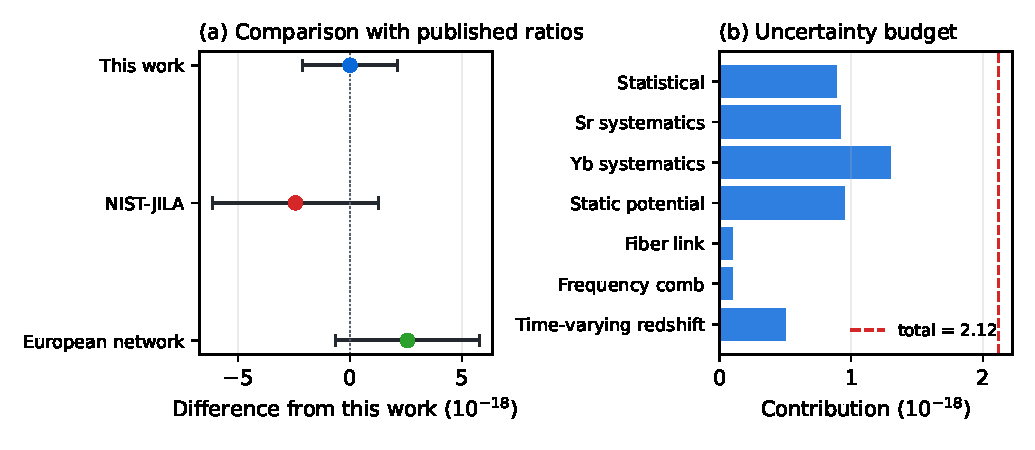
\includegraphics[width=\linewidth]{figs/fig3_compare.pdf}
  \caption{Comparison and budget. (a) Differences between this work and
  the published Yb/Sr ratios, with their quoted uncertainties.
  (b) Components of the total standard uncertainty; the dashed line marks
  the quadrature total.}
  \label{fig:compare}
\end{figure}

Changes in the Earth's gravitational potential enter the comparison
directly. The static difference between the two clock transitions is
fixed by first-order spirit leveling and is carried in the uncertainty
budget; of the time-varying contributions, the tidal term is carried as
a data-driven uncertainty item, while co-seismic steps from the
regional seismicity during the campaign fall well below the reported
precision. At this accuracy, it is the geodetic determination of the
potential difference, rather than its variability, that limits the
comparison; the same sensitivity underlies proposed
chronometric-geodesy applications of optical-clock
networks~\citep{grotti2018geodesy, takamoto2020redshift,
mcgrew2018geodesy}.

The treatment of the time-varying term illustrates this point.
Applying the supplied tide series as a template correction leaves the
residual segment scatter larger, not smaller
(Section~\ref{sec:results-budget}): a tidal model that is adequate for
geophysical purposes is not necessarily adequate at the $10^{-18}$
level, where ocean-tide loading, hydrological mass redistribution and
their local phase and amplitude errors all
matter~\citep{voigt2016timevariable}. A correct time-dependent
treatment would require a dedicated geodetic campaign with in-situ
gravimetry and site-specific loading models; that is beyond the scope
of this paper and is left to future work. Until such a treatment
exists, the reported ratio carries the time-varying term
conservatively in its uncertainty budget.

The campaign also demonstrates the operational character that a
future optical-clock network will need. Over the two-month campaign
the two clocks were restarted, the transfer chain re-locked, and the
beat record interrupted many times; the segment-level ratio estimates
show no evidence of a systematic offset between the three measuring
stages, so the reproducibility of the comparison does not depend on
continuous operation of either system. This is the practical
counterpart of the coordinated multi-clock
campaigns~\citep{lindvall2025coordinated, pizzocaro2026european}: the
network tolerates interruption, provided each retained window is
self-consistently characterized.

Several limitations bound the present result. First, the per-segment
statistical uncertainties from the Allan-deviation extrapolation are
the dominant budget term, and five of the sixteen segments carry
model-limited fits; the random-effect treatment accounts for their
excess scatter at the level of the reported uncertainty, but a longer
record would reduce the statistical term. Second, the systematic
evaluations of the two clocks are those published by the
laboratories; independent verification of those budgets, as opposed
to the transfer, is not attempted here. Third, the geopotential
difference is taken from a first-order leveling campaign; an
alternative value exists in the experiment records and is carried as
an external item pending reconciliation, as is the physical-model
provenance of the supplied tide series and the exact accounting of
the full sample totals. Finally, the present campaign meets the
uncertainty requirement of the roadmap but not the full criterion,
which additionally requires each ratio to be measured at least twice
by different institutes and repeated over an extended period.

Looking ahead, the result establishes this link as a prototype node
pair of a distributed optical-clock network: the same infrastructure
can be extended to further nodes, and the technique demonstrated here
-- clocks at different sites agreeing at the redefinition threshold --
is the operation that both the redefinition and post-redefinition
applications require. The building blocks for such a network are now
in place: terrestrial fiber links of the kind used
here~\citep{schioppo2022cavities, chen2026dissemination} carry
comparisons over thousands of kilometers within continents, while
free-space and satellite-based links are closing the remaining
gaps~\citep{shen2021satellite, caldwell2023geo, shen2022freespace,
pizzocaro2021vlbi}. The natural next step is a hybrid architecture in
which optical-clock nodes on continental fiber backbones are
interconnected across oceans by satellite or free-space optical links,
so that any pair of clocks on Earth can be compared at the level
demonstrated here. Realizing it will put the same demands on geodetic
infrastructure that this comparison
faced~\citep{grotti2018geodesy, mcgrew2018geodesy}.
